\chapter[DSB-SC using multiplier IC AD633]{DSB-SC using multiplier IC AD633}
\label{chapdsbsc}
\section*{Aim}
To set up a balanced modulator circuit for double side band suppressed carrier amplitude modulator.
\section*{Theory}
DSB-SC is a kind of amplitude modulation in which the carrier frequency component is absant. It is generated by multiplying the carrier and maodulating signals. If $e_c$ is the carrier and $e_m$is the message signal, where
\begin{equation}
e_c=E_c\  sin\ 2\pi f_ct
\end{equation}
\begin{equation}
e_m=E_m\  sin\ 2\pi f_mt
\end{equation}
Multiplication is done using AD633 (See \ref{AD633}) multiplier IC.
Applying $e_m$ to $\textbf{X}$ and $e_c$ to $\textbf{Y}$ with $\textbf{Z}$ is grounded, 
\begin{equation}
W= \frac{e_me_c}{10} =\frac{Emsin(2\pi f_mt).Ecsin(2\pi f_ct)}{10}
\end{equation}
\begin{equation}
W= \frac{E_mE_c}{10} \frac{[cos 2\pi (f_c\ -\ f_m)t-cos 2\pi (f_c\ +\ f_m)t]}{2}
\end{equation}
\begin{equation}
W= \frac{E_mE_c [cos 2\pi (f_c\ -\ f_m)t]}{20}- \frac{E_mE_c[cos 2\pi (f_c\ +\ f_m)t]}{20}
\end{equation}
This wave contains both the sidebands at $f_c-f_m$ and $f_c+f_m$, but not the wave at carrier frequency\footnote{$sin \ A.\ sin\ B=\frac{cos\ (A-B)-cos\ (A+B)}{2}$}. Hence the name double sideband suppressed carrier modulation(DSB-SC).

The following figure \ref{DSBSC} shows\footnote{By Serych at cs.wikipedia [Public domain], from Wikimedia Commons.  \ \url{http://commons.wikimedia.org/wiki/File\%3AAM-DSBSC.png}} the DSB-SC signal in blue and the original message is shown in red. (\emph{It is an indicative graph, not to scale as per the experimental set-up.})
\begin{figure}[h]
\begin{center}
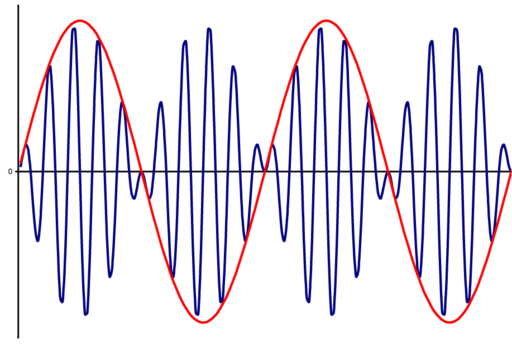
\includegraphics[width=10cm,height=4cm]{AMDSBSC.png}
\caption{DSB-SC signal in blue, original message shown in red.}
\label{DSBSC}
\end{center}

\end{figure}

Multiplying the DSB-SC with the carrier once again will result in the following output.
\begin{equation}
\begin{split}
W=\frac{1}{10} &[ \frac{E_mE_c [cos (2\pi (f_c\ -\ f_m)t)]}{20} \\
&\quad -\frac{E_mE_c[cos (2\pi (f_c\ +\ f_m)t)]}{20}].
 E_c sin(2\pi f_ct)
\end{split}
\end{equation}

\begin{equation}
\begin{split}
W=& \frac{E_m.{E_c}^2}{400}sin(2\pi (2f_c-f_m)t)  -  \frac{E_m.{E_c}^2}{400}sin(2\pi (2f_c+f_m)t)\\ 
&\quad +\frac{E_m.{E_c}^2}{200}sin(2\pi f_mt)
\end{split}
\end{equation}
Thus the signal consists of various frequencies of which, the smallest is the message frequency. It can be extracted by filtering using a low pass filter. Since the amplitude of the message frequency is very small, It may be amplified using a simple non-inverting amplifier using an opamp.

%%%%%%%%%%%%%%%%%%%%%%%%%%%%%%%%%%%
\begin{figure}[ht]
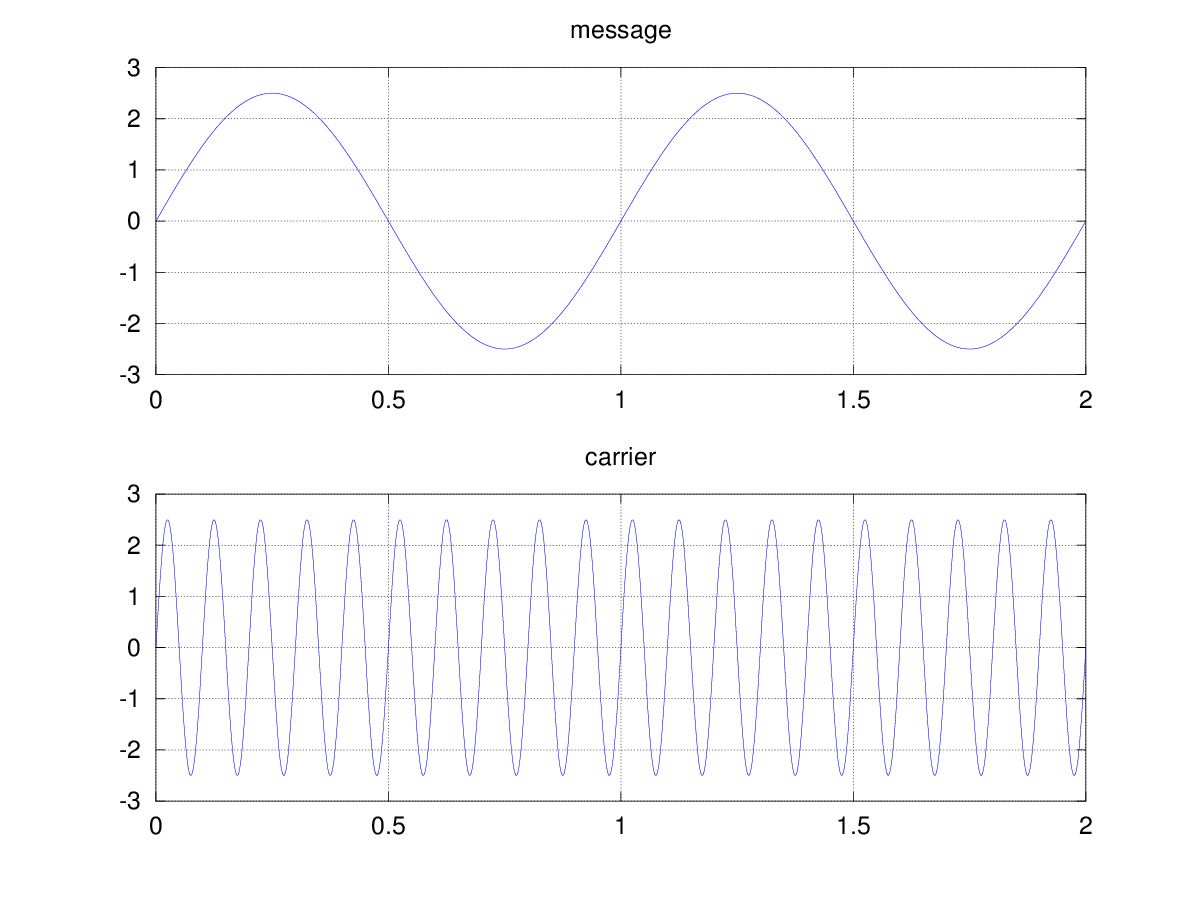
\includegraphics[width=\textwidth]{am6331.png}
\caption{Message and carrier signals}
\label{msg633plot1}
\end{figure}
%%%%%%%%%%%%%%%%%%%%%%%%%%%%%%%%%%%%
\section*{Design}

To the \textbf{X} input of the IC, feed the message sinusoid of amplitude $E_m=2.5\ V$ and frequency $f_m= 1\ kHz$.\\

To the \textbf{Y} input of the IC, feed the carrier sinusoid of amplitude $E_c=2.5\ V$ and frequency $f_c= 100\ kHz$.\\
Ground the \textbf{Z} input of the IC.\\
Provide the biasing voltage of +15 V to pin 8 of the IC and -15 V to pin 5 of the IC.\\

The output signal will have a waveform as given by,

\begin{equation}
W=\frac{X.Y}{10}+Z
\end{equation}
\begin{equation}
W=\frac{e_m.e_c}{10}=\frac{(2.5) \ .(2.5)}{10}\frac{[cos 2\pi99kt-cos 2\pi101kt]}{2}
\end{equation}

\begin{equation}
W=\frac{6.25}{20}[cos 2\pi99kt-cos 2\pi101kt]
\end{equation}

 This is the DSB-SC waveform.
 
 \begin{figure}[ht]
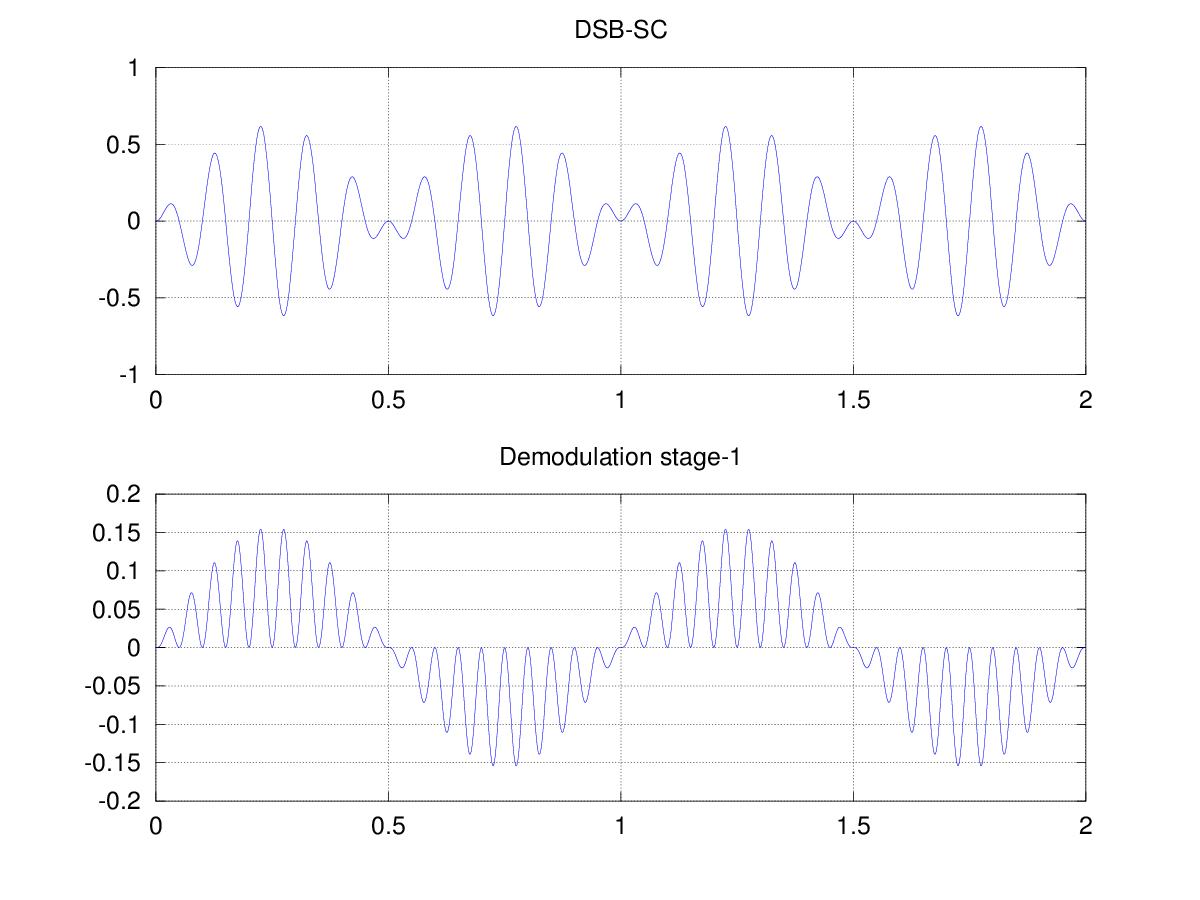
\includegraphics[width=\textwidth]{dsbsc6332.png}
\caption{AM(DSB-FC) and Demodulation stage-1 signals}
\label{dsbsc633plot2}
\end{figure}
 
 \paragraph{Demodulation}  is by multiplying the DSB-SC signal once again with the carrier. This can be implemented by connecting another AD633 IC in cascade with the first one.

\noindent The multiplication will result in the following output, as per the theory already explained.

\begin{equation}
\begin{split}
W=& \frac{15.625}{200}sin(2\pi 1kt)\\
&\quad  +\frac{15.625}{400}sin(2\pi199kt) -\frac{15.625}{400}sin(2\pi 201kt)
\end{split}
\end{equation}

\noindent This waveform is shown in Figure \ref{dsbsc633plot2}, which is the stage -1 in demodulation. The next step is to obtain the message signal. This is done by lowpass filtering the above signal at a cut-off frequency of 1.5 kHz.

To design an RC lowpass filter of cut-off frequency 1kHz,

\begin{equation}
f_c=\frac{1}{2\pi R_1C_1}=1.5kHz
\end{equation}
Choose $C_1=0.01\  \mu F$
$\therefore  R_1 =7.5 \ k \Omega$

A non-inverting amplifier may be used to amplify this signal. Using a feedback resistor of $R_f= 100 \ \k Omaga$ and an input resistance of $R_i=10\ k\Omega$ will result in a gain of $A_v=1+\frac{R_f}{R_i}=11$.
\begin{sidewaysfigure}[ht]
    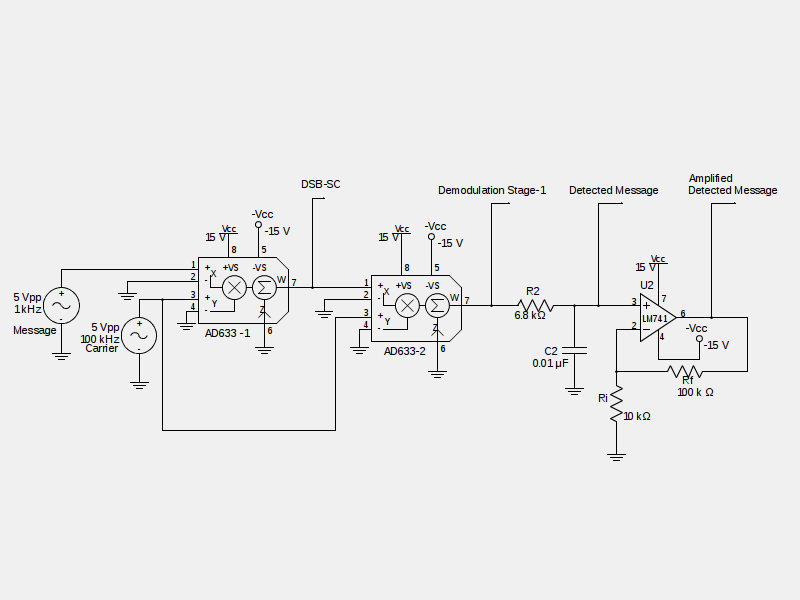
\includegraphics[scale=0.8, trim=0cm 4cm 0cm 4cm,clip=true]{633dsbsc.png}
    \caption{Circuit for DSB-SC generation and detection using AD633 multiplier IC}
    \label{DSBSCckt}
\end{sidewaysfigure}


\section*{Circuit Diagram}
The circuit diagram for implementing DSBSC using multiplier IC is shown in figure \ref{DSBSCckt}.




\section*{Procedure}
\begin{itemize}
\item
Make connections as shown in the circuit diagram, figure \ref{DSBSCckt}.
\item
Feed the message and carrier signals.
\item
Connect the pin number 7 of the IC to a CRO and observe the resultant waveform which is DSB-SC.
\item
Connect the pin number 7 of the second IC to a CRO and observe the resultant waveform which is the product of DSB-SC and the carrier.(Named demodulation stage-1 signal)
\item
Observe the output from the filter, amplified by the opamp amplifier, which extracts the envelope -\emph{The 1kHz message signal}- of the previous signal.
\item
Plot the signals observed on a graph sheet.
\end{itemize}
\section*{Observation}



The input and output signals as observed on a CRO are shown in Figure \ref{msg633plot1} and \ref{dsbsc633plot2}.


\section*{Result}
Implemented DSB-SC using multiplier IC AD 633 and observed the signal waveforms.